\documentclass[hyperref={pdfpagelabels=false}]{beamer} 

\usepackage[portrait]{sfocs-poster}
\usepackage{lipsum}
\usepackage{rotating}
\usebackgroundtemplate{%
	% image as background
		\tikz\node[opacity=0.9] {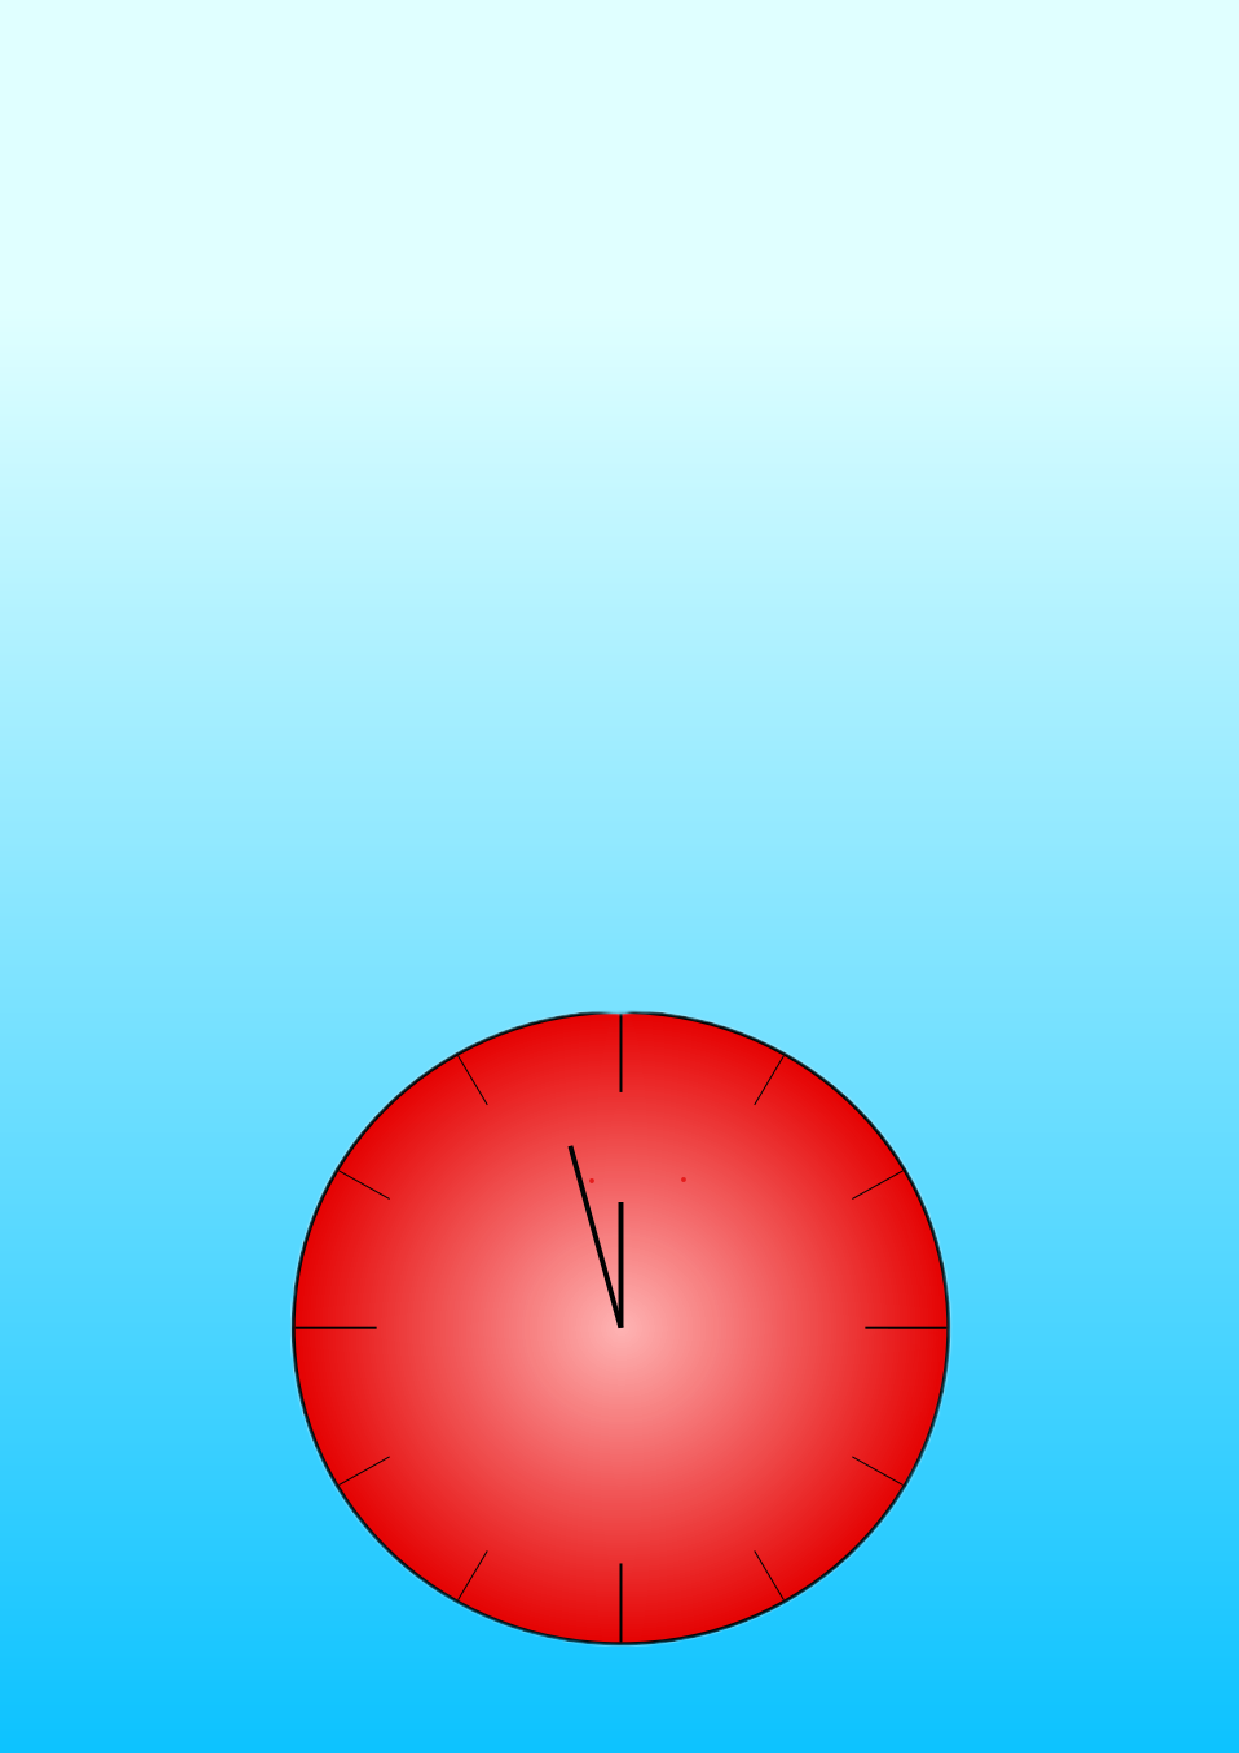
\includegraphics[height=\paperheight,width=\paperwidth]{img/pg}};
	% plain color 
	%\tikz[remember picture,overlay] \fill[game] (current page.north west) rectangle (current page.south east); 
}
%
% sample boxes 
% 
\tcbset{
        framedbox/.style={
					enhanced, fontupper=\large,left=.75cm,fonttitle=\LARGE,toptitle=.25cm,bottomtitle=.25cm,halign title=center
        },
}

\newtcolorbox{basebox}[3][]{framedbox,coltitle=#2,colback=#3,coltext=#2,title=#1,colframe=#3,sharp corners}
\newtcolorbox{baseroundedbox}[3][]{framedbox,colback=#3,colframe=#3,coltitle=#2,coltext=#2,title=#1,,rounded corners,arc=15pt}
\newtcolorbox{transparentbox}[4][]{framedbox, colback=#3,colbacktitle=#3,colframe=#3,coltitle=#2,coltext=#2,title=#1,frame style={color=#3},opacitybacktitle=#4,opacityback=#4,opacityframe=#4,opacityfill=#4}
\newtcolorbox{blankbox}{blanker,fontupper=\LARGE}


% draw a grid
%\beamertemplategridbackground[0cm]

\begin{document}

\begin{frame}

	\begin{textblock}{45}(2,1)
		\begin{blankbox}
			
\includegraphics[width=1000pt]{img/gamename.png} \\\hspace*{\fill} \\ \\
		\end{blankbox}
	\end{textblock}


\begin{turn}{60}
	\begin{textblock}{1}(67,3)
		\begin{blankbox}
			\centering
			
\includegraphics[height=200pt]{img/aLine}
		\end{blankbox}
	\end{textblock}
\end{turn}


\begin{textblock}{20}(71,3.8)
		\begin{blankbox}
			\Huge\textbf{MINIMALISM}

\vspace{0.4cm}

			\textbf{SIMPLICITY}
\vspace{0.4cm}

\textbf{ENTERTAINMENT}
		\end{blankbox}
	\end{textblock}



\begin{textblock}{10}(1.3,15)
		\begin{blankbox}
			\centering
			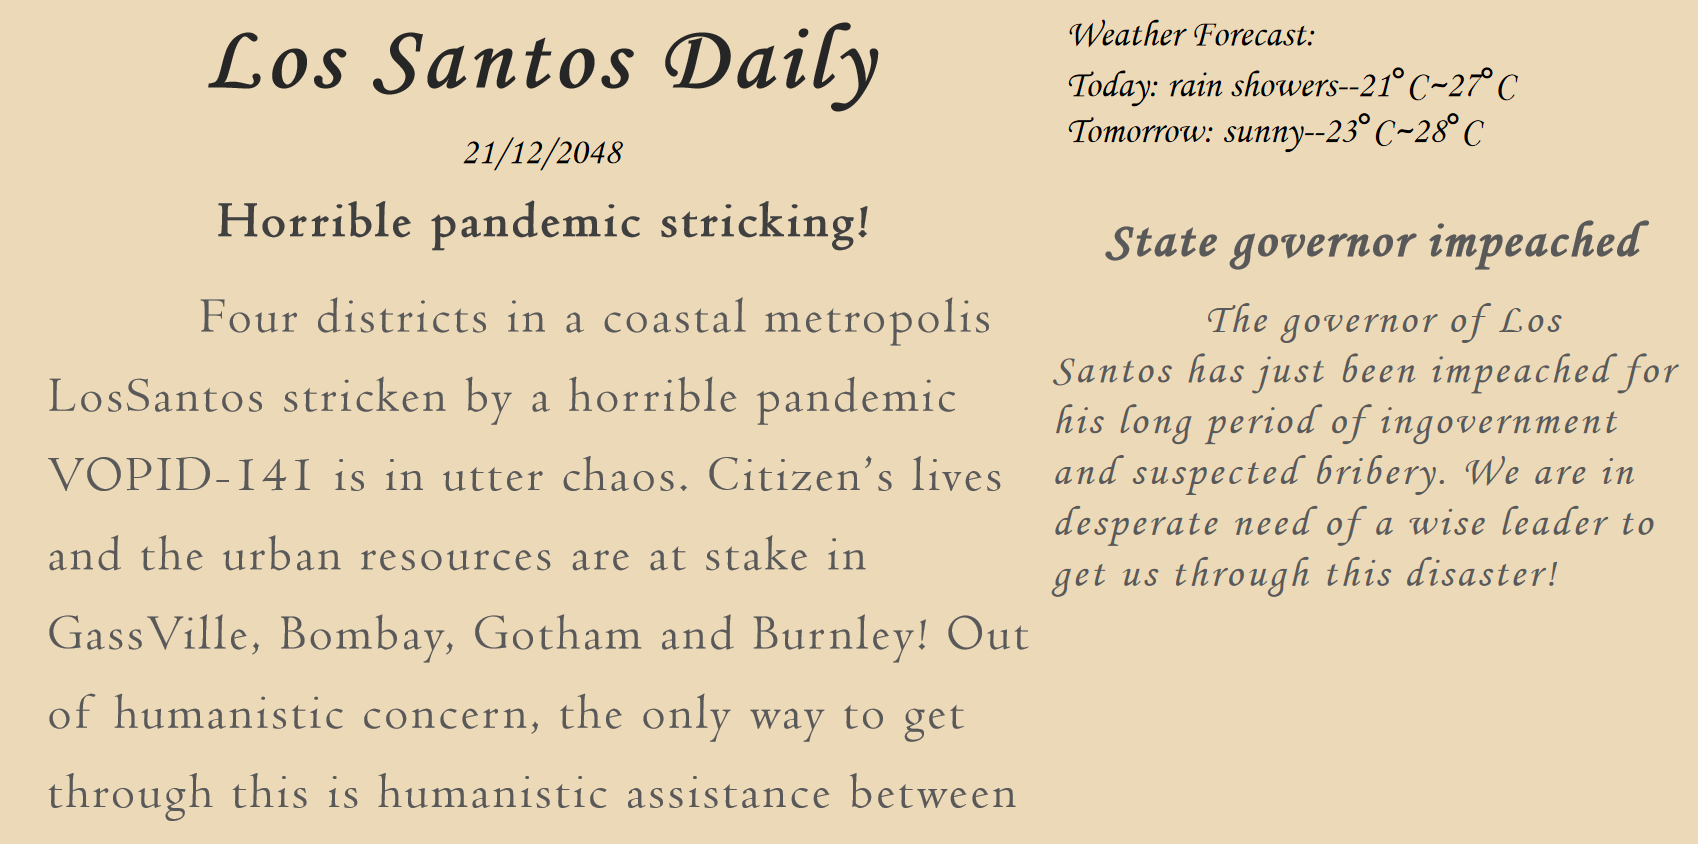
\includegraphics[angle=8,height=525pt]{img/news.png}
		\end{blankbox}
	\end{textblock}




	\begin{textblock}{40}(58,16)
		\begin{blankbox}
\vspace {0.4cm}
The clock is ticking, so the players are pressed to make moral decisions balncing the safety of districts by tranfering the CR (Critical Resources) lightning fast.The goal of this game is to find the impact of differtent CR on each CPs thus only transfer the CR most effectivelyly. Alternatively, any CPs hitting 0 would instantly indicate failure.\vspace {0.4cm}

 Terminator recreates for the players the scenario where countless medical workers, policy makers and all the other concerned parties had to make tough decisions facing extremelystressful situations just to save our lives and protect our countries as best as they can during the real pandemic COVID-19 last year. May their great spirit inspire us.\vspace {0.4cm}
			
		\end{blankbox}
	\end{textblock}





\begin{textblock}{35}(1,42)
		\begin{blankbox}
		\huge \textbf{ Brief Instructions On The Game} 
						\begin{itemize}
							\item \textbf {Local CP}
							\item Health Threat Drop: People infected in an area -- rise after good decisions
							\item \textbf {Global CP}
							\item Citizen Trust: The faith citizens have on player -- rise after good decisions
							\item External Safety: Safety of the areas you govern -- drop after bad decisions
							\item Disposable Money: Financial support of fighting virus -- drop after bad decisions
						\end{itemize}
			
		\end{blankbox}
	\end{textblock}


\begin{textblock}{40}(38,42)
		\begin{blankbox}
			\centering
			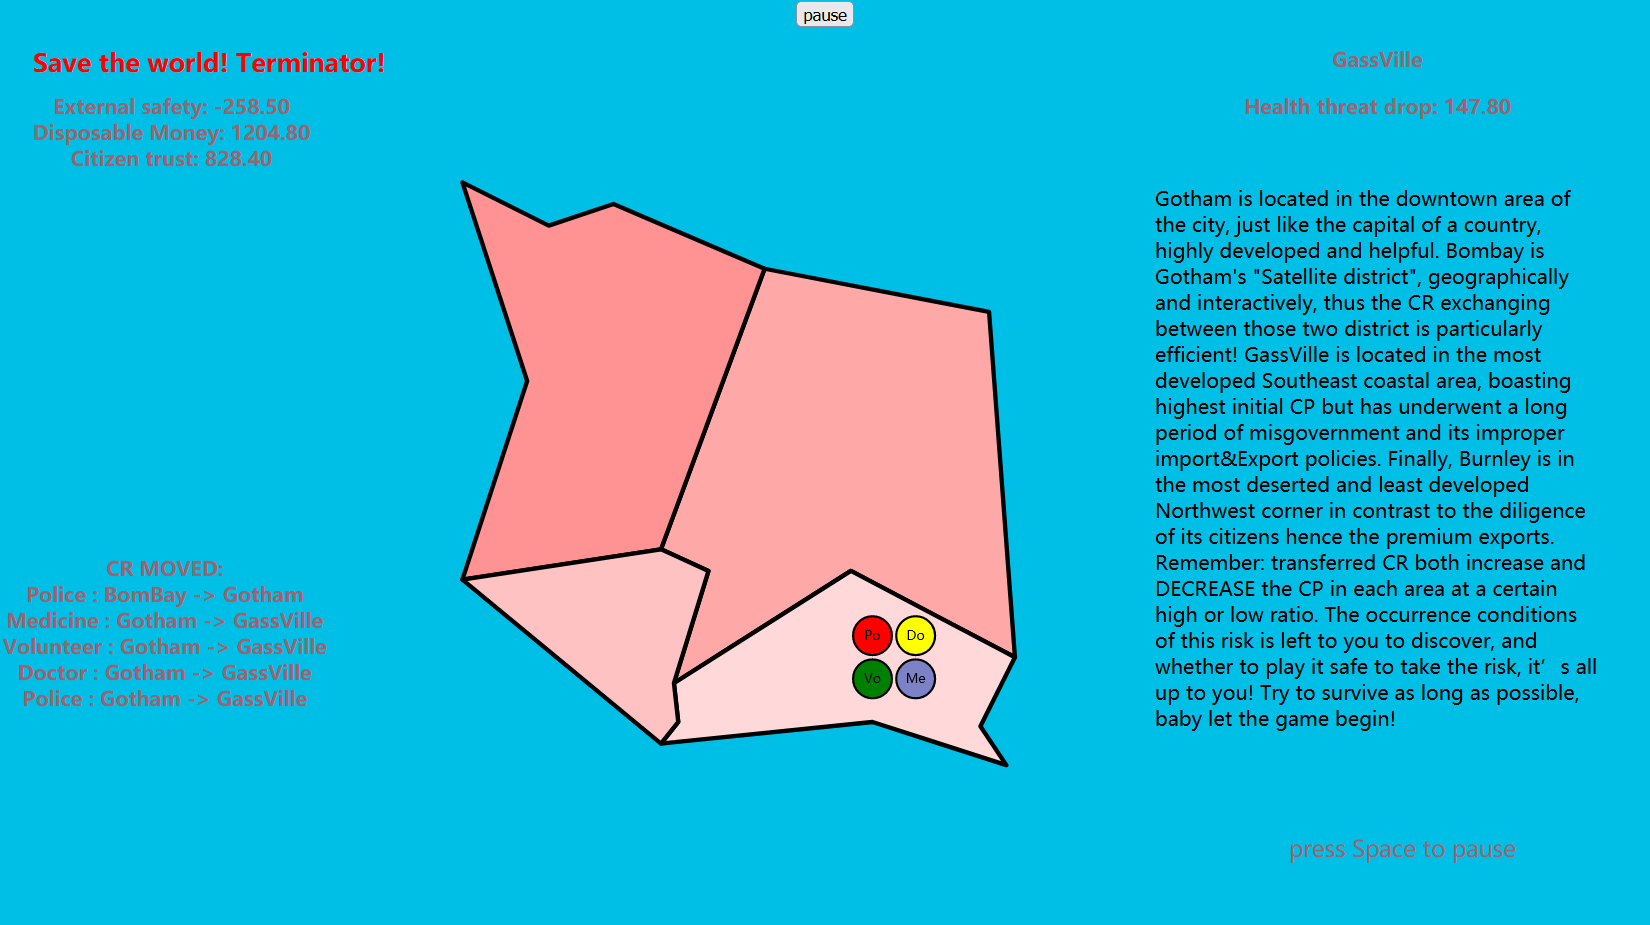
\includegraphics[ height=570pt]{img/newDemo}
		\end{blankbox}
	\end{textblock}



	% #1: box width 
	% #2 #3: coordinates on percent 


	
	\begin{textblock}{50}(25.5,70)
		% no title provided, extra parameter is opacity in [0,1] 		
		\begin{transparentbox}{black}{red}{.2}
				\vspace{.25cm}
				\centering\huge\textbf{Main Appeal}\vspace{1cm}

\begin{itemize}\itemsep .85cm
			{ \item Highly Customized User Control

				\item Simple yet ingenious Operation

				\item Engaging Humanism Concept

				\item  Diverse Gaming Mods}
\end{itemize}       	 

		\end{transparentbox}
	\end{textblock} 




\begin{textblock}{50}[1,1](75.5,90)
		\begin{blankbox}
			
			\centering {\textbf{The current pandemic has inspired this game.\\
\vspace{.25cm}
Become a protagonist and a savior!}}
			
		\end{blankbox}
	\end{textblock}

	% option [0,1] means box anchor is bottom left	
	\begin{textblock}{80}[0,1](1,100)
		\logos[light]
	\end{textblock}

	% option [1,1] means box anchor is bottom right	
	\begin{textblock}{45}[1,1](97,100)
		\begin{blankbox}
			\huge\textbf{{THREE TO ONE:}} 
			\Large{Zining Wang (C),
			Yifan Jia,
			Qiao Liu }
			
		\end{blankbox}
	\end{textblock}

	\begin{textblock}{10}(10,70)
		\begin{blankbox}
			\centering
			
\includegraphics[height=400pt]{img/ai97b-ej97b.png}
		\end{blankbox}
	\end{textblock}

	\begin{textblock}{10}(80,70)
		\begin{blankbox}
			\centering
			
\includegraphics[height=400pt]{img/arn28-kj5eh.png}
		\end{blankbox}
	\end{textblock}

	



	\begin{textblock}{30}(28,92.5)
		\begin{blankbox}
			
\includegraphics[width=205pt]{img/Teamlogo.png}

		\end{blankbox}
	\end{textblock}



\end{frame}

\end{document}

transparent box 
larger title font 
no gradient 
plain box
